% Name: Labeled contour lines
% Description: Level curves of f(x, y) = x^2/4 + y^2 at f = 1, 2, 3, and 4, each labeled with its value, and the gradient at one point, perpendicular to its curve.
% Tags: contour plot, level curves, gradient, multivariable calculus

\usepackage{pgfplots}
\pgfplotsset{compat=1.18}

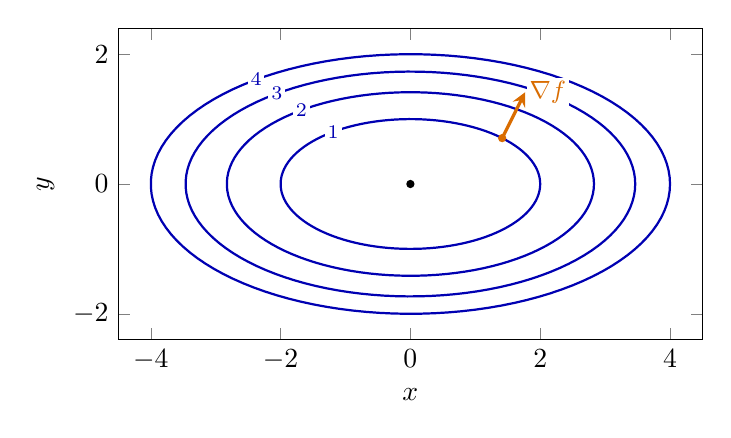
\begin{tikzpicture}[lvl/.style={pos=0.375, fill=white, inner sep=1pt, font=\scriptsize, text=blue!70!black}]
  \begin{axis}[
    width=9cm, height=5.6cm, axis equal image,
    xmin=-4.5, xmax=4.5, ymin=-2.4, ymax=2.4,
    xlabel=$x$, ylabel=$y$, domain=0:360, samples=120,
  ]
    % The level f = c is the ellipse x = 2 sqrt(c) cos t, y = sqrt(c) sin t.
    \pgfplotsinvokeforeach{1,2,3,4}{
      \addplot[blue!70!black, thick] ({2*sqrt(#1)*cos(x)}, {sqrt(#1)*sin(x)}) node[lvl] {$#1$};
    }
    \fill (axis cs:0,0) circle (1.5pt);
    % At (sqrt 2, 1/sqrt 2) on f = 1 the gradient (x/2, 2y) is (0.707, 1.414); drawn at half length.
    \draw[-stealth, very thick, orange!85!black] (axis cs:1.414,0.707) -- (axis cs:1.768,1.414) node[right, fill=white, inner sep=1pt, font=\small] {$\nabla f$};
    \fill[orange!85!black] (axis cs:1.414,0.707) circle (1.5pt);
  \end{axis}
\end{tikzpicture}
